\let\negmedspace\undefined
\let\negthickspace\undefined
\documentclass[journal]{IEEEtran}
\usepackage[a5paper, margin=10mm, onecolumn]{geometry}
%\usepackage{lmodern} % Ensure lmodern is loaded for pdflatex
\usepackage{tfrupee} % Include tfrupee package

\setlength{\headheight}{1cm} % Set the height of the header box
\setlength{\headsep}{0mm}     % Set the distance between the header box and the top of the text

\usepackage{gvv-book}
\usepackage{gvv}
\usepackage{cite}
\usepackage{amsmath,amssymb,amsfonts,amsthm,mathtools}
\usepackage{algorithmic}
\usepackage{graphicx}
\usepackage{textcomp}
\usepackage{xcolor}
\usepackage{txfonts}
\usepackage{listings}
\usepackage{enumitem}
\usepackage{mathtools}
\usepackage{gensymb}
\usepackage{comment}
\usepackage[breaklinks=true]{hyperref}
\usepackage{tkz-euclide} 
\usepackage{listings}
\def\inputGnumericTable{}                                 
\usepackage[latin1]{inputenc}                                
\usepackage{color}                                            
\usepackage{array}                                            
\usepackage{longtable}                                       
\usepackage{calc}                                             
\usepackage{multirow}                                         
\usepackage{hhline}                                           
\usepackage{ifthen}                                           
\usepackage{lscape}
\begin{document}

\bibliographystyle{IEEEtran}
\vspace{3cm}

\title{3.2.13}
\author{EE24BTECH11002 - Agamjot Singh}
% \maketitle
% \newpage
% \bigskip
{\let\newpage\relax\maketitle}

\renewcommand{\thefigure}{\theenumi}
\renewcommand{\thetable}{\theenumi}
\setlength{\intextsep}{10pt} % Space between text and floats

\textbf{Question:}
\newline
Draw a triangle $\vec{ABC}$ in which $\vec{AB} = 5 cm$, $\vec{BC} = 6 cm$ and $\angle\vec{ABC} = 60\degree$.
\newline
\textbf{Solution:}
\newline
\begin{table}[h!]    
	\centering
	\begin{tabular}[12pt]{ |c| c|}
    \hline
    \textbf{Variable} & \textbf{Description}\\ 
    \hline
	$\vec{A}$ & Point to be found\\
    \hline
	$\vec{B}$ & $(0, 0)$ point\\
    \hline
	$\vec{C}$ & $(6, 0)$ point\\
    \hline
	$\vec{\angle \vec{ABC}}$ & $60 \degree$\\ 
    \hline
    \end{tabular}
	\caption{Variables Used}
	\label{tab1-1.5-29}
\end{table}\\
The rotation matrix \brak{\vec{P}} is given by,
\begin{align}
	\vec{P} = \myvec{\cos{\theta} & -\sin{\theta}\\\sin{\theta} & \cos{\theta}}
\end{align}
where $\theta$ is the angle rotated in anti-clockwise direction.
\newline
The coordinates of $\triangle ABC$ can then be expressed as
\begin{align}
	\vec{B} &= \myvec{0\\0}, \vec{C} = \myvec{6\\0}, \vec{A} = \norm{\vec{AB}}\vec{P}\brak{\frac{\vec{BC}}{\norm{\vec{BC}}}}\\
	\implies \vec{A} &= \norm{\vec{B} - \vec{A}}\myvec{\cos{\theta} & -\sin{\theta}\\\sin{\theta} & \cos{\theta}}\frac{\brak{\vec{C} - \vec{B}}}{\norm{\vec{C} - \vec{B}}}\\
	\implies \vec{A} &= 5\myvec{\frac{1}{2} & \frac{-\sqrt{3}}{2}\\\frac{\sqrt{3}}{2} & \frac{1}{2}}\myvec{1\\0}\\
	\implies \vec{A} &= \myvec{\frac{5}{2}\\\frac{5\sqrt{3}}{2}}
\end{align}

\begin{figure}[h!]
   \centering
   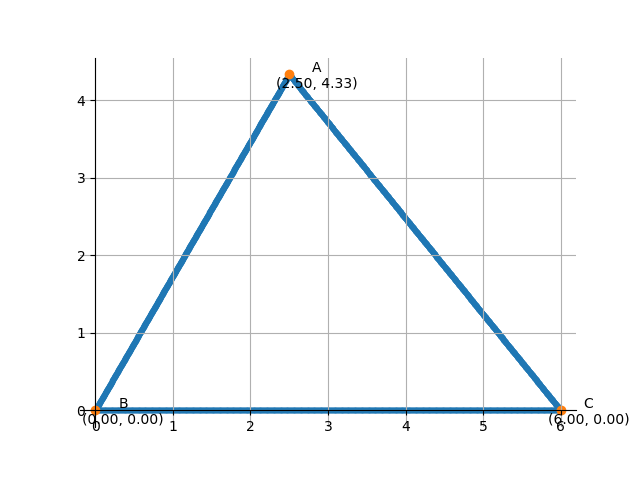
\includegraphics[width=0.7\linewidth]{figs/graph.png}
   \caption{Graph representing $\triangle \vec{ABC}$}
\end{figure}

\end{document}
